\documentclass{beamer}
\usepackage[utf8]{inputenc}
\usepackage{amsmath, amssymb, bm}
\usepackage{physics}
\usepackage{graphicx}
\usepackage{hyperref}
\usepackage{xmpmulti}
\usepackage{tikz}
\usepackage{pgfplots}
\pgfplotsset{compat=newest}
\usepackage{siunitx}
\usepackage{longtable}
\sisetup{round-mode=places,round-precision=1}
\usepackage{braket}
\usetikzlibrary{arrows.meta, shapes.misc, positioning, backgrounds}
\usetikzlibrary{calc, decorations.markings,decorations.pathmorphing}
\usetheme{Madrid} % You can change the theme as you like
\usecolortheme{seagull}
%\renewcommandCopy{\qty\SI} 



\begin{document}

\title{Reinforcement Learning (classical and quantum) for Quantum Control}
\author{Morten Hjorth-Jensen}
\institute{Department of Physics, UiO, Norway}
\date{February 2026}


%-----------------------------------------------------------
%\begin{frame}
%    \titlepage
%\end{frame}

%-----------------------------------------------------------


\begin{frame}[plain,fragile]
\frametitle{Inspiration}

\begin{alertblock}{Inspiration}
\begin{itemize}
\item {\bf Reinforcement Learning for Quantum Technlogy}, by Marin Bukov and Florian Marquardt, arXiv:2601.18953
\item {\bf Model-aware reinforcement learning for high-performance Bayesian experimental design in quantum metrology}, by Federico Belliardo, Fabio Zoratti, Florian Marquardt, and Vittorio Giovannetti, Quantum 8, 1555 (2024)
\item {\bf Hybrid quantum-classical reinforcement learning in latent observation spaces}, Daniel T. R. Nagy, Csaba Czaban, Bence Bako, Peter Haga, Zsófia Kallus, and Zoltan Zimborás  Quantum Machine Intelligence {\bf 7}, 88 (2025).
\end{itemize}
\end{alertblock}

\end{frame}

\begin{frame}[plain,fragile]
\frametitle{Many-body physics, Machine Learning, Quantum Machine Learning and Quantum Control}

\begin{block}{}
\begin{itemize}
\item 
\item 
\item 
\end{itemize}
\end{block}

\end{frame}



\begin{frame}[plain,fragile]
\frametitle{Di Vincenzo criteria}

\begin{alertblock}{Quantum computing requirements }
\begin{enumerate}
\item A scalable physical system with well-characterized qubit

\item The ability to initialize the state of the qubits to a simple fiducial state

\item Long relevant quantum coherence times longer than the gate operation time

\item A universal set of quantum gates

\item A qubit-specific measurement capability
\end{enumerate}
\end{alertblock}
\end{frame}

\begin{frame}
\frametitle{Our platform, electrons on helium}
  {
      
	
      \begin{footnotesize}
     \begin{columns}
       \column{5.0cm}
\begin{alertblock}{EEROQ and MSU}
\begin{enumerate}
\item Long coherence times

\item Highly connect qubits

\item Many qubits in a small area

\item CMOS compatible

\item Fast gates
\end{enumerate}
\end{alertblock}
\column{6cm}
      \begin{center}
	\rotatebox[origin=c]{-90}{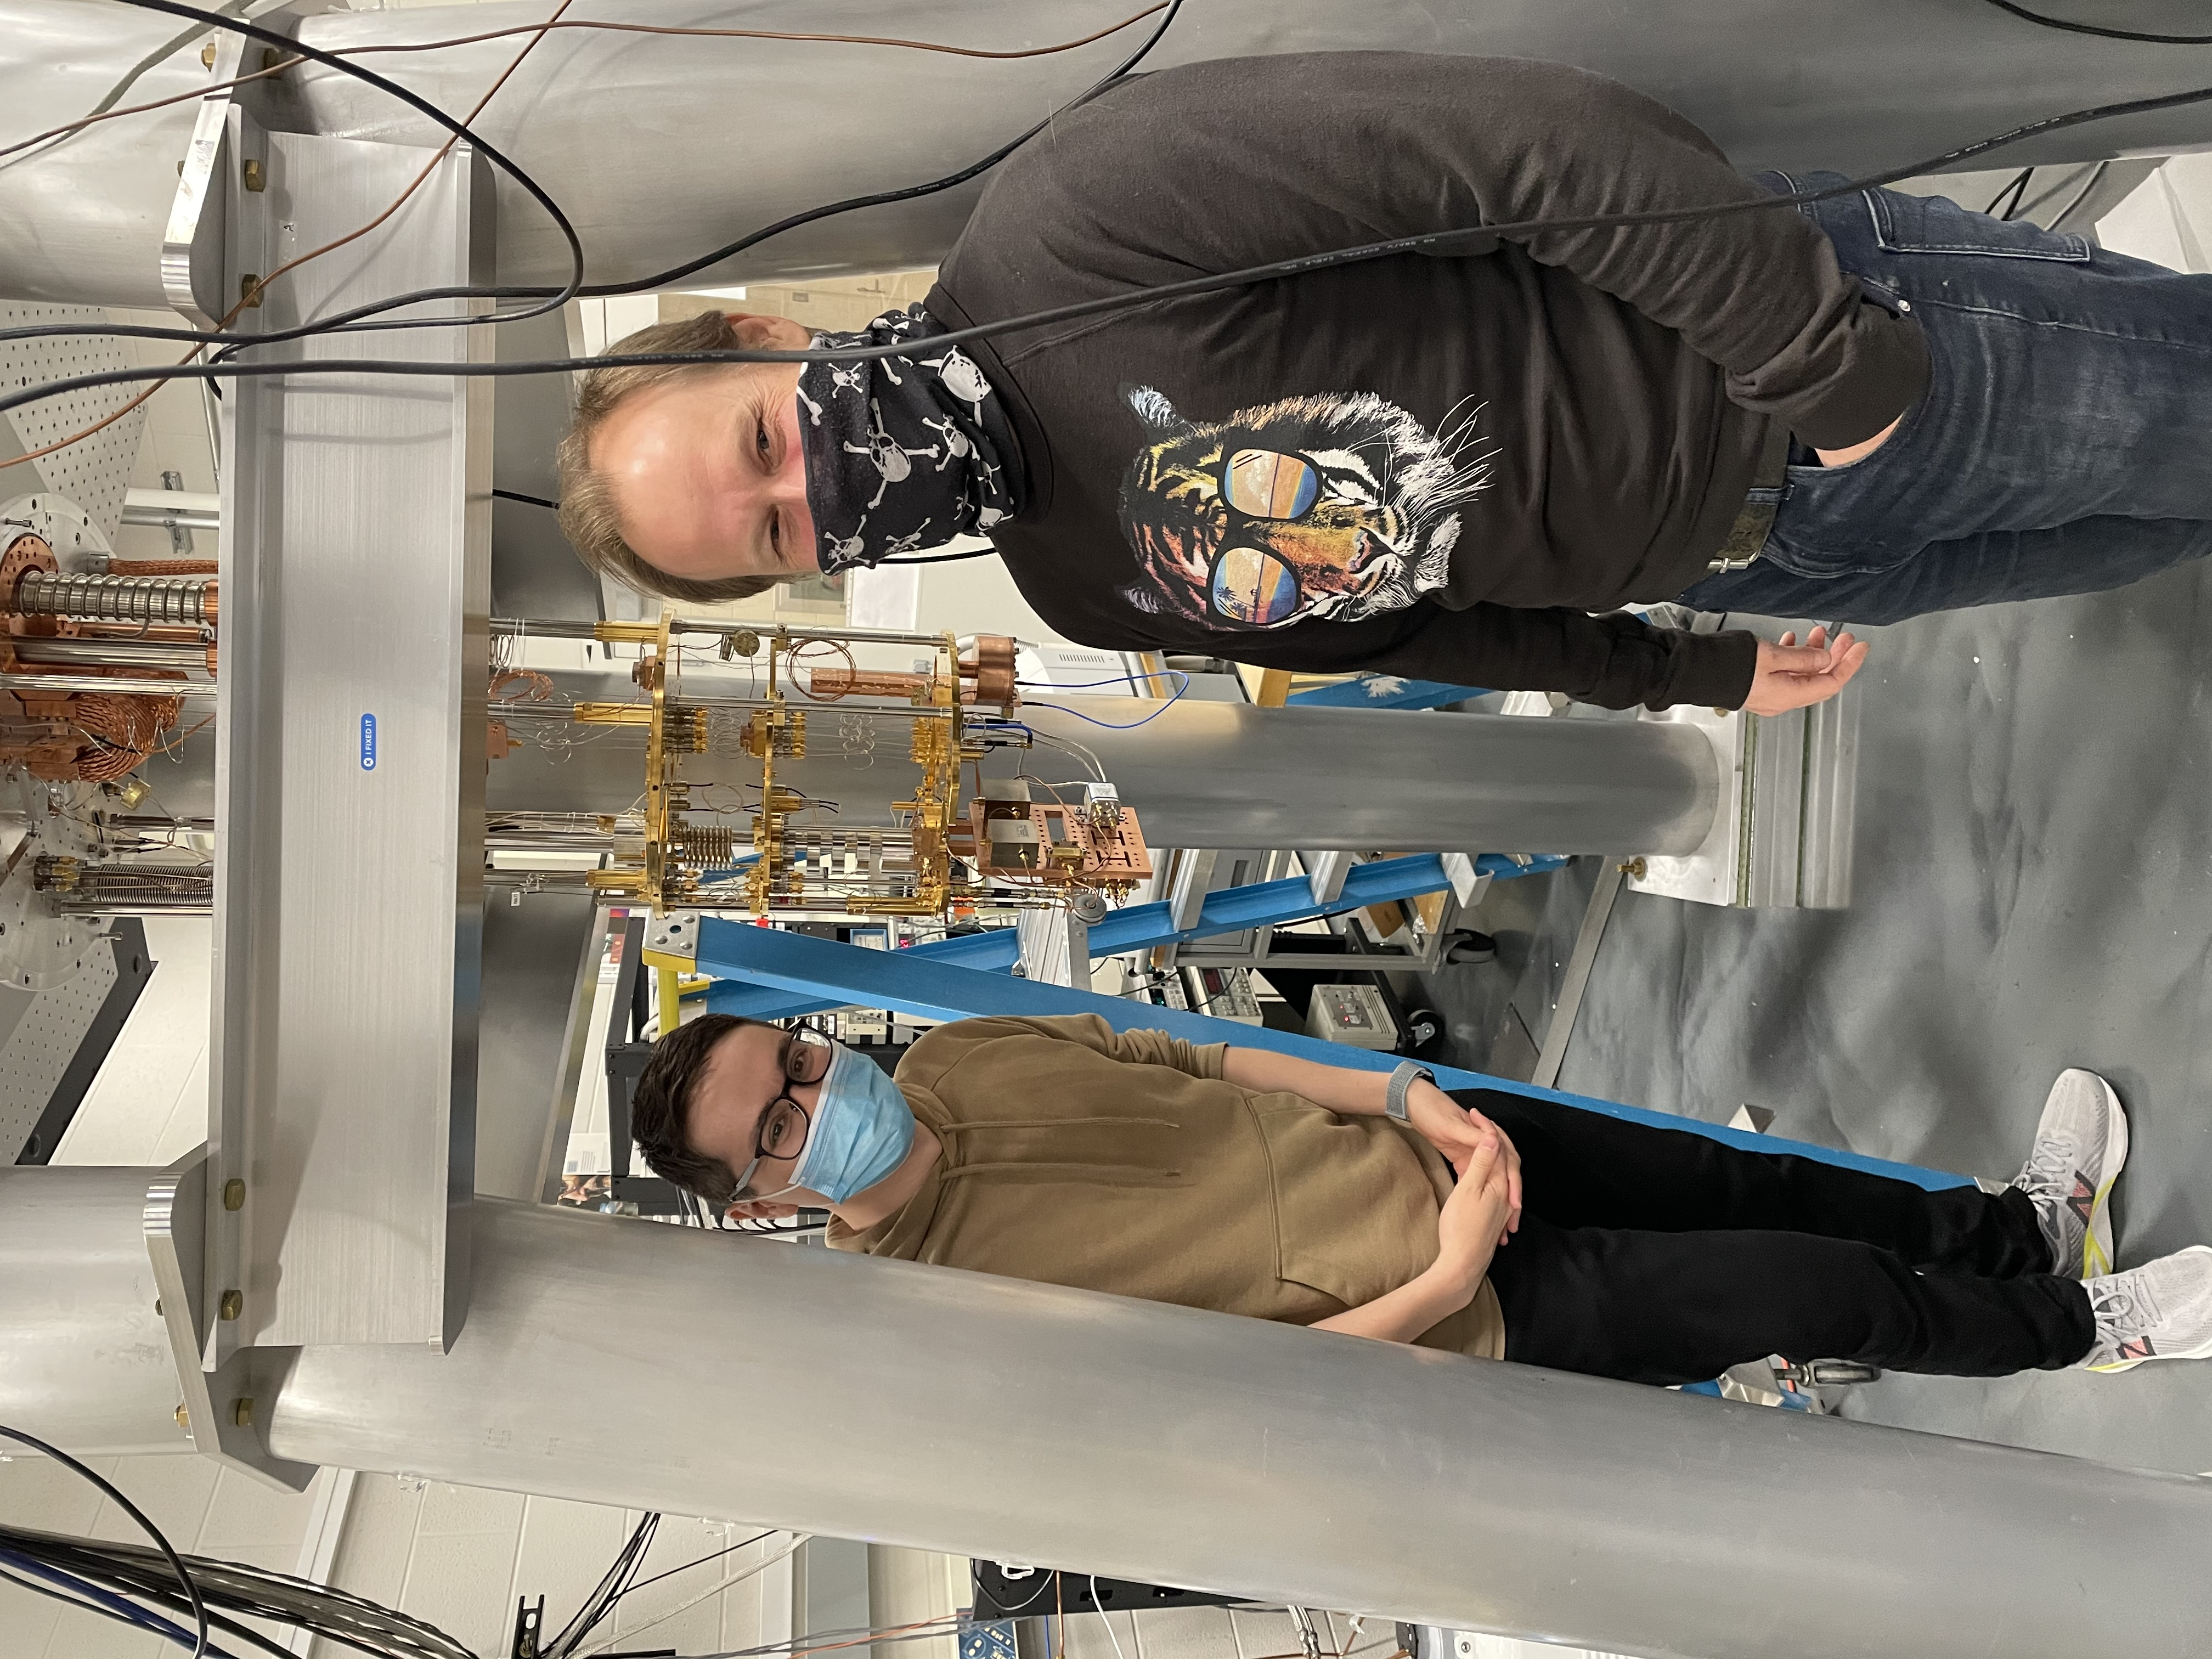
\includegraphics[width=1.3\textwidth]{qcfigures/lab.jpeg}}
      \end{center}
\end{columns}
      \end{footnotesize}
    }
\end{frame}
\begin{frame}[plain,fragile]





\begin{frame}[plain,fragile]
\frametitle{Neural quantum states, PINNs and quantum PINNs: harmonic oscillator quantum dot}

\begin{block}{Quantum Neural Networks and PINNs}
%\begin{table*}[t]
\footnotesize{
  \centering
%  \begin{threeparttable}
    \begin{tabular}{c|c|c|cc|cc}
      \toprule
      $N$ & $\omega$ & DMC & PINN+BF & \%\,err & PINN+CTNN & \%\,err \\
      \midrule
      2 & 0.001 & --- & $0.0137948(8)$ & --- & $\mathbf{0.013778(1)}$ & --- \\
    & 0.01 & ---            & $0.69125(2)$  & --- & $\mathbf{0.69036(1)}$ & --- \\
    & 0.10 & $3.55385(5)$   & $3.5549(1)$   & $+0.0295$ & $\mathbf{3.55388(5)}$ & $+0.0008$ \\
    & 0.50 & $11.78484(6)$  & $11.7895(4)$  & $+0.0395$  & $\mathbf{11.7847(2)}$ & $-0.0000$ \\
    & 1.00 & $20.15932(8)$  & $20.1610(6)$  & $+0.0083$  & $\mathbf{20.1585(3)}$ & $-0.0041$ \\
    \midrule
    12 & 0.001 & ---          & $0.515823(3)$ & --- & $\mathbf{0.515365(4)}$ & --- \\
    & 0.01 & ---           & $2.48620(5)$  & --- & $\mathbf{2.47363(4)}$ & --- \\
    & 0.10 & $12.26984(8)$ & $12.2731(2)$  & $+0.0160$ & $\mathbf{12.2718(1)}$ & --- \\
    & 0.50 & $39.1596(1)$  & $39.1786(8)$  & $+0.0485$ & $\mathbf{39.1604(3)}$ & $+0.0018$ \\
    & 1.00 & $65.7001(1)$  & $65.717(1)$   & $+0.0257$ & $\mathbf{65.69556(5)}$ & $-0.0069$ \\
    \midrule
    20 & 0.001 & ---          & --- & --- & $\mathbf{1.293033(6)}$ & --- \\
    & 0.01 & ---           & ---  & --- & $\mathbf{6.14645(5)}$ & --- \\
    & 0.10 & $29.9779(1)$ & ---  & --- & $29.9888(2)$ & $+0.0364$ \\
    & 0.50 & $93.8752(1)$  & ---  & --- & $\mathbf{93.8789(5)}$ & $+0.0040$ \\
    & 1.00 & $155.8822(1)$  & ---   & --- & $\mathbf{155.8738(7)}$ & $-0.0024$ \\
    \bottomrule
\end{tabular}
%\end{threeparttable}
%\end{table*}}
\end{block}

\end{frame}

\begin{frame}[plain,fragile]
\frametitle{Parametric Matrix Models, Trotterization, Unitary CC and quantum computing}
      \begin{footnotesize}
     \begin{columns}
       \column{5.0cm}
       \begin{alertblock}{Parametric matrix models}
         \begin{itemize}
           \item   Parametric matrix models (PMMs) as a way to compute the Lie-Trotter formula,
             see Nature Communications {\bf 16}, 5929 (2025), Cook, Jammooa, MHJ, Lee and Lee
           \item Extrapolated Trotter approximation for quantum computing simulations. We plot the lowest three energies of the effective Hamiltonian for the one-dimensional Heisenberg model with DM interactions versus time step $dt$. All training (diamonds) and validation (circles) samples are located away from dt = 0.
         \end{itemize}
\end{alertblock}       
\column{5cm}
      \begin{center}
	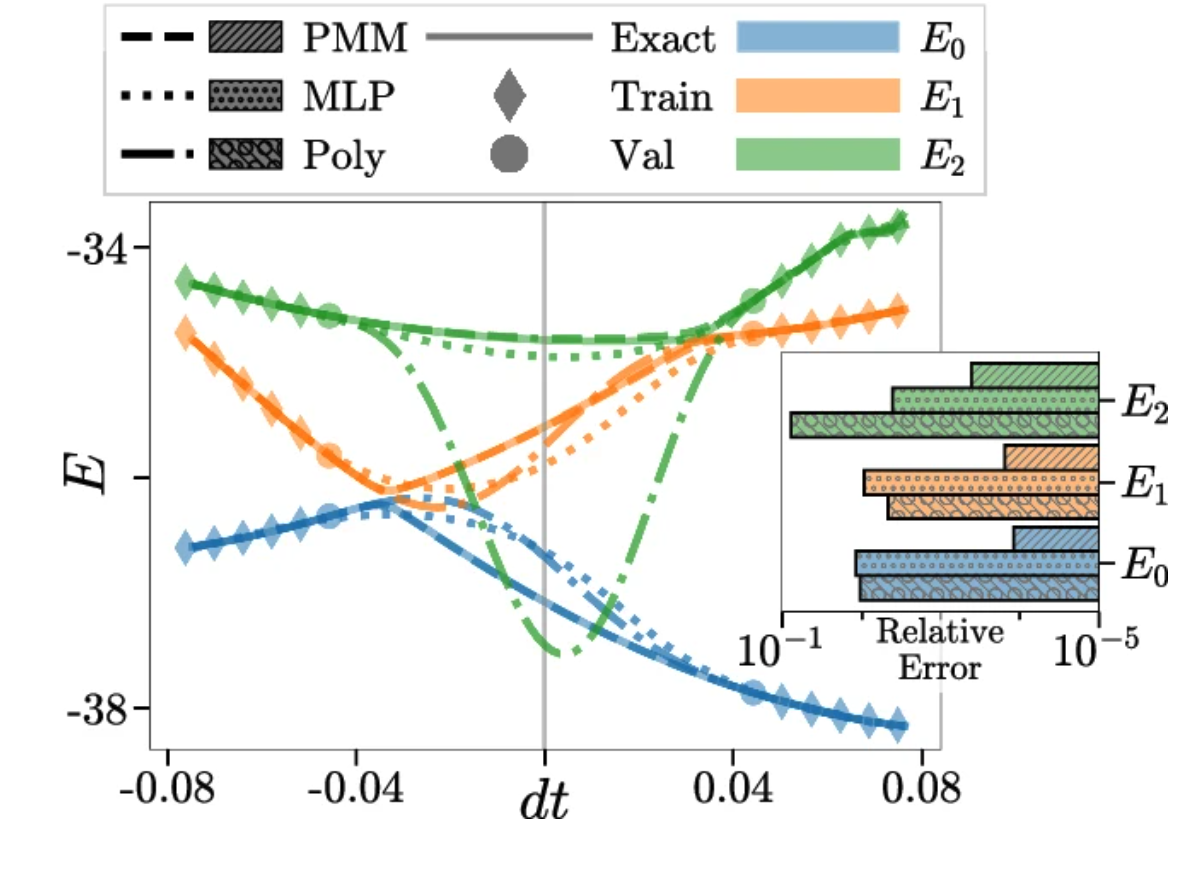
\includegraphics[width=1.2\textwidth]{qcfigures/trotter.png}
      \end{center}
\end{columns}
      \end{footnotesize}
    }
\end{frame}


\begin{frame}[plain,fragile]
\frametitle{Qauntum sensing: Singlet-triplet leakage for entangled electrons on helium}

%\vspace{6mm}

\centerline{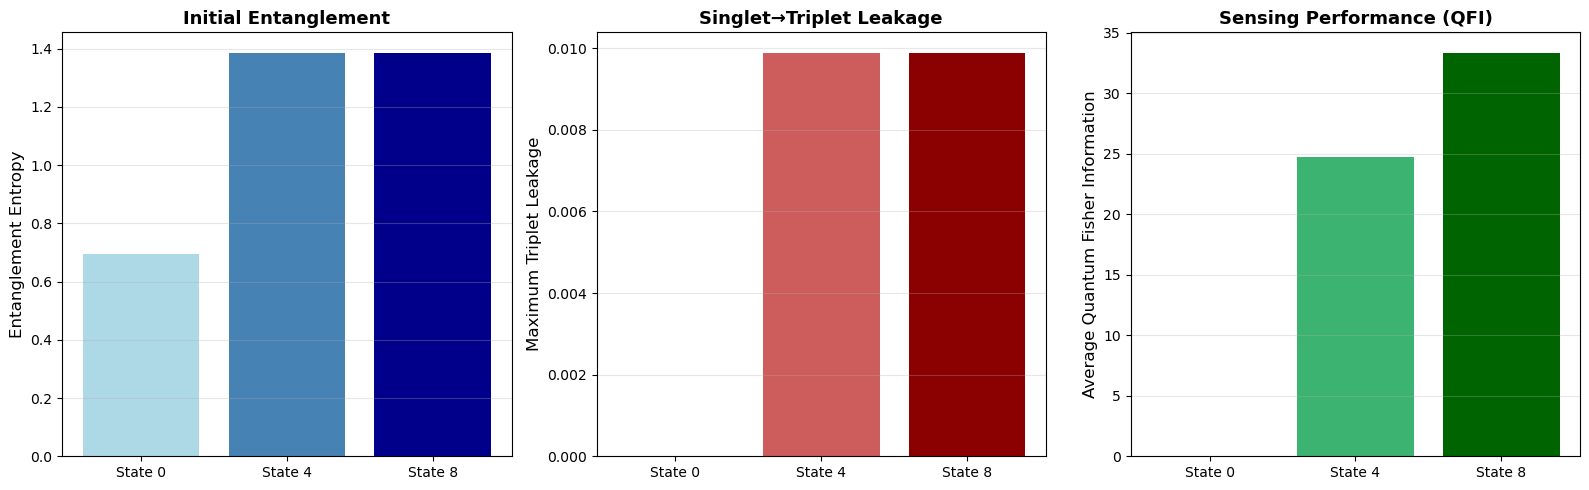
\includegraphics[width=1.0\linewidth]{qcfigures/figure_008.png}}

%\vspace{6mm}
\end{frame}


\begin{frame}[plain,fragile]{Reinforcement Learning for Optimal Quantum Control}

W are implementing a \textbf{model-based reinforcement learning} approach to optimize the control sequence for quantum sensing. Since we \textbf{know the Hamiltonian}, we can simulate the quantum dynamics and use RL to find optimal control strategies.

\end{frame}

\begin{frame}[plain,fragile]{RL Framework:}

\begin{alertblock}{Sequential Decision Process}
\begin{itemize}    
\item \textbf{State}: $(t, |\psi(t)\rangle, \mu_\phi, \sigma_\phi^2)$ - time, quantum state, posterior mean & variance of phase
\item \textbf{Action}: $(B_{\text{amp}}, t_{\text{pulse}}, V_{\text{trap}})$ - magnetic field amplitude, pulse duration, trap voltage
\item  \textbf{Transition}: Evolve under $B(t)\sigma_z^{(1)} + V_{\text{trap}}(x,y)$ and kinetic plus Coulomb
\item \textbf{Measurement}: Projective measurement in singlet/triplet basis
\item \textbf{Reward}: Quantum Fisher Information of final state
\end{itemize}
\end{alertblock}
\textbf{Goal}: Maximize cumulative QFI over multiple measurement cycles to achieve optimal phase estimation.

\end{frame}

\begin{frame}[plain,fragile]{Physical Interpretation}

\begin{alertblock}{What we've shown:}
\begin{itemize}
\item \textbf{Singlet-Triplet Oscillations}: The magnetic field $B(t)$ on one electron causes the initially pure singlet state to oscillate between singlet and triplet components. This "leakage" is directly measurable through spin-selective detection.
\item \textbf{Phase-Dependent Signal}: The triplet population depends on the accumulated phase $\phi(t) = \int_0^t B(t') dt'$, providing a way to measure the time-integrated field.

\item \textbf{Quantum Fisher Information}: Quantifies how sensitive our entangled state is to the phase. Higher QFI means:
\begin{itemize}
\item Better precision in estimating $\phi$ (and thus $B(t)$)
\item Approach to the Heisenberg limit of quantum metrology
\item Advantage over classical (separable state) sensors
\end{itemize}
\end{itemize}
\end{alertblock}
\end{frame}

\begin{frame}[plain,fragile]{Physical Interpretation}

\begin{alertblock}{What we've shown:}
\begin{itemize}
\item \textbf{Excited States vs Ground State}: We use an \textbf{excited singlet state with maximum entanglement} rather than the ground state because:
\begin{itemize}
\item Higher entanglement → stronger quantum correlations
\item More sensitive response to perturbations
\item Enhanced quantum Fisher information
\item Better phase estimation precision
\item The comparison shows QFI scales with entanglement!
\end{itemize}
\item  \textbf{Applications}:
\begin{itemize}
\item \textbf{Magnetic field sensing}: Detect weak, time-varying magnetic fields
\item \textbf{NMR/ESR spectroscopy}: Enhanced signal detection
\item \textbf{Quantum metrology}: Fundamental limits of measurement precision
\item \textbf{Quantum information}: Characterizing decoherence and noise
\end{itemize}
\end{itemize}
\end{alertblock}
\end{frame}

\begin{frame}[plain,fragile]{Physical Interpretation}
\begin{alertblock}{Key result}

Highly-entangled excited singlet states are superior quantum sensors
compared to weakly-entangled ground states. The singlet to triplet
leakage provides a direct readout of the magnetic field, with
sensitivity quantified by the quantum Fisher information!
\end{alertblock}
\end{frame}




\end{document}















